\begin{frame}{\textit{Redes de Distribuição}}
  \begin{block}{Modelo Tradicional}
    \begin{itemize}
      \item Grandes geradoras de energia, geralmente próximas às fontes
      primárias de energica
      \item Energia produzida e transmitida aos grandes centros, para então ser
      distribuída aos consumidores
    \end{itemize}
  \end{block}
  \begin{figure}[h]
  	\begin{center}
      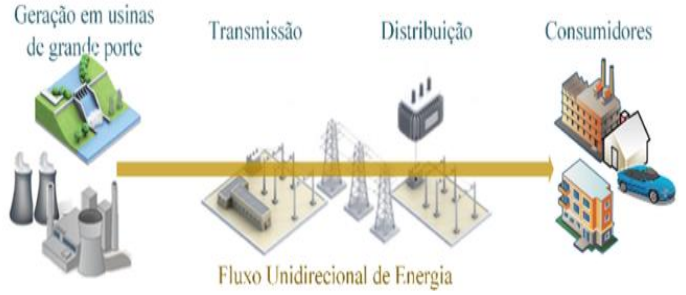
\includegraphics [scale=0.333]{./Figures/TraditionalGrid}
      %\caption {Valores da Tarifa Branca - CELPA (Fonte:}
  		%\label{fig:arq-imuno}
  	\end{center}
  \end{figure}
\end{frame}

\begin{frame}{Redes de Distribuição}
  \begin{block}{Modelo de Rede Inteligente - \textbf{\textit{Smart Grid}}}
    \begin{itemize}
      \item Integração de \alert{TIC} para fins de monitoramento e tráfego de
      informações
      \item Alto grau de \alert{automação} da rede de distribuição
      (confiabilidade/flexibilidade)
      \item \alert{Interação do consumidor} com a rede de distribuição:
      \begin{itemize}
        \item Ciente e participativo com relação ao consumo
        \item Gerenciamento pelo lado da demanda
        \item Geração de energia pelo lado da demanda (geração distribuída)
      \end{itemize}
    \end{itemize}
  \end{block}
  \begin{figure}[h]
  	\begin{center}
      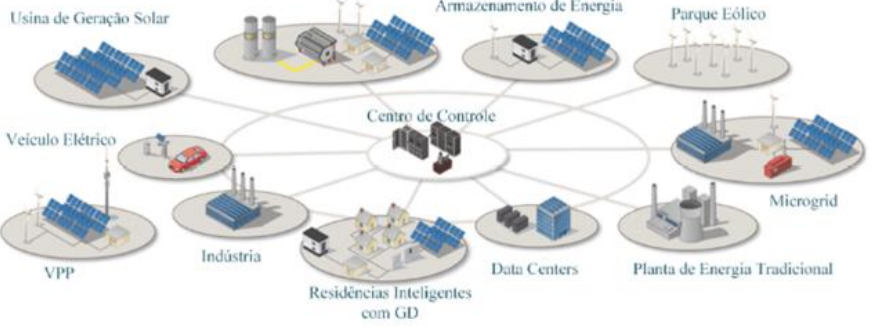
\includegraphics [scale=0.27]{./Figures/SmartGrid}
      %\caption {Valores da Tarifa Branca - CELPA (Fonte:}
  		%\label{fig:arq-imuno}
  	\end{center}
  \end{figure}
\end{frame}

\begin{frame}
  \begin{block}{Gerenciamento pelo lado da Demanda}
    \begin{itemize}
      \item Modifica perfil de consumo através de incentivos financeiros
      \item Busca um consumo de acordo com o perfil desejado, e não uma geração
      de acordo com a demanda
      \item Diversas técnicas propostas na literatura:
      \begin{itemize}
        \item Preços dinâmicos (ex: Tarifa Branca)
        \item Controle e escalonamento da utilização de equipamentos pela
        distribuidora
      \end{itemize}
    \end{itemize}
  \end{block}
\end{frame}

\begin{frame}
  \begin{figure}[h]
  	\begin{center}
      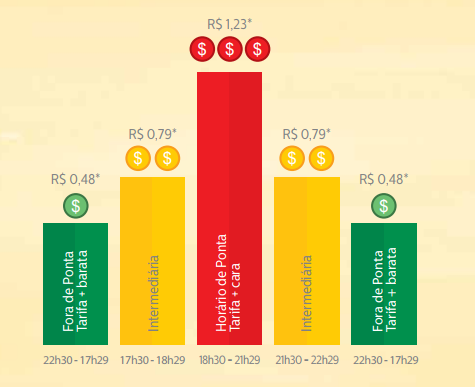
\includegraphics [scale=0.7]{./Figures/TarifaBranca}
      \caption {Valores da Tarifa Branca - CELPA (Fonte:
      http://www.celpa.com.br/imobiliario/simuladores/consumo-de-energia-na-tarifa-branca).}
  		%\label{fig:arq-imuno}
  	\end{center}
  \end{figure}
\end{frame}

\begin{frame}
  \begin{block}{Consumo doméstico}
    \begin{itemize}
      \item Utensílios domésticos possuem alto consumo:
      \begin{itemize}
        \item Lava louças, lava roupas, secadora, etc ...
      \end{itemize}
      \item Podem sobrecarregar a rede em caso de uso simultâneo
      \item Controle sobre o escalonamento destes equipamentos podem evitar
      as sobrecargas
    \end{itemize}
  \end{block}
  \pause
  \begin{block}{Algoritmos de Escalonamento propostos na Literatura}
    \begin{itemize}
      \item Abordagens:
      \begin{itemize}
        \item \textit{Particle Swarm Optimization} (PSO)
        \item Altoritmos evolucionários (GA)
        \item \textit{Cuckoo Search algorithm} (CSA)
      \end{itemize}
    \end{itemize}
  \end{block}
\end{frame}

\begin{frame}
  Neste trabalho, cargas domésticas são escalonados pelo CSA visando o
  balanceamento da curva de carga da rede, levando em consideração as o máximo
  possível as preferências dos usuários
  \begin{block}{Considerações}
    \begin{itemize}
      \item Agendamento considera a carga do transformador, e não da residência
      \item 4 consumidores
      \item 5 cargas comutáveis por consumidor
      \item Algoritmo de escalonamento ótimo baseado em CSA
      \item Resultados comparados com otimizador baseado em AG
    \end{itemize}
  \end{block}
\end{frame}

%\begin{frame}
%  \begin{block}{}
%    \begin{itemize}
%      \item
%    \end{itemize}
%  \end{block}
%\end{frame}

%\begin{frame}
%  \begin{block}{}
%  \end{block}
%\end{frame}

%\begin{frame}
%  \begin{figure}[h]
%  	\begin{center}
%      \includegraphics [scale=0.3]{./Figures/Device-Estimates}
%     % \caption {Estimativa de dispositivos conectados à Internet.}
%  		%\label{fig:arq-imuno}
%  	\end{center}
%  \end{figure}
%\end{frame}

%\begin{frame}{Redes de Acesso}
%	\begin{figure}[!htb]
%		\centering
%		\subfloat[DSL]{
%			\includegraphics[height=3.5cm]{./Figures/DSLaccess}
%			\label{figdroopy}}
%		\quad %espaco separador
%		\subfloat[Cable]{
%			\includegraphics[height=3.5cm]{./Figures/CableAccess}
%			\label{figsnoop}}
%		%\caption{Subfiguras}
%		%\label{fig01}
%	\end{figure}
%\end{frame}

%\begin{frame}[fragile]
%\scriptsize
%\begin{verbatim}
%\end{verbatim}
%\end{frame}

%\begin{frame}{\textit{Socket Programming with TCP}}
%\scriptsize
%\lstinputlisting[language=Python, caption={TCP Server.}]{./code/upperServer/TCPserver.py}
%\end{frame}
